\section{Decisiones de diseño}
Al inicializar la clase \texttt{RegEx} generamos su AFD mínimo respectivo 
y lo guardamos en un nuevo atributo llamado \texttt{\_afd} para luego al hacer cada 
\texttt{match} poder usarlo y no tener que generarlo cada vez.

Para varios de los algoritmos que implementamos decidimos usar los sets de Python. De todas formas, estos sets tienen limitaciones,
el mayor limitante es la incapacidad de crear sets con elementos no hasheables, lo cual nos seria de gran utilidad al necesitar sets de sets en los algoritmos de nuestra solucion. 
Ademas, otro impedimento es el hecho de que no se puede iterar un set y agregar o sacar valores en el medio de la iteración. Para resolver el primer problema utilizamos, 
cuando es necesario los frozensets, conjuntos que son hashables al no ser modificables, y para resolver el segundo utilizamos listas, aunque también podríamos haber utilizado una cola,
ya que cumple con las operaciones que necesitamos en el algoritmo de determinización.

Decidimos tratar a los autómatas como inmutables luego de inicializarlos así que en determinizar, en minimizar y al sacar los 
estados inaccesibles creamos nuevos autómatas en vez de modificar los ya existentes.

\section{Eleccion de algoritmos}
Al generar el AFND a partir de la expresión regular utilizamos el algoritmo de Thompson basandonos 
en la inducción del teorema visto en clase. Se puede decir que en la implementación extendemos el invariante 
con tener los estados del autómata normalizados en cada paso.

Para hacer la minimización, vimos en clase los algoritmos de Moore, Brzozowski y de Hopcroft. 
De estos usamos el de Hopcroft porque tiene la mejor complejidad temporal, $O(ns \log{n})$ 
y porque se basa en hacer operaciones entre conjuntos, las cuales ya tenemos implementadas con los sets de Python.
Este algoritmo requiere que el autómata no tenga estados inaccesibles, por lo tanto en el método \texttt{minimize}  
de la clase AFD que primero creamos un autómata equivalente sin estados inaccesibles y luego aplicamos el algoritmo de Hopcroft sobre el mismo.

\section{Benchmarks}
Para comparar nuestra solución con la naive decidimos utilizar la expresión regular $r = a^*$, sobre el alfabeto $\Sigma = \{a, b\}$. A continuación mostramos el
tiempo que tardaron en ejecutarse ambos programas con cadenas aleatorias sobre $\Sigma^*$ de longitudes $10, 100$ y $1000$ y con cantidades de cadenas $10, 100, 1000, 10000, 100000$ y $1000000$,
en milisegundos. Las columnas indican la cantidad de cadenas y las filas indican las longitudes de las cadenas.

\begin{center}
\begin{tabular}{|l|l|l|l|l|l|l|}
\multicolumn{7}{c}{Solución naive} \\ \hline
     & 10 & 100 & 1000 & 10000 & 100000 & 1000000 \\ \hline
10   & 65ms & 76ms & 80ms & 110ms & 513ms & 4.47s \\
100  & 71ms & 74ms & 114ms & 444ms & 4.31s & 37.24s \\
1000 & 69ms & 127ms & 585ms & 5.16s & 49.32s & 8min 34s \\ \hline
\end{tabular}
\end{center}

\begin{center}
\begin{tabular}{|l|l|l|l|l|l|l|}
\multicolumn{7}{c}{Nuestra solución} \\ \hline
     & 10 & 100 & 1000 & 10000 & 100000 & 1000000 \\ \hline
10   & 68ms & 73ms  & 74ms & 81ms & 214ms & 1.20s \\
100  & 68ms & 65ms & 78ms & 91ms & 199ms & 1.29s \\
1000 & 71ms & 71ms & 68ms & 95ms & 306ms & 2.91s \\\hline
\end{tabular}
\end{center}

Para generar cadenas aleatorias creamos un programa en \texttt{/tlengrep/cadenas\_de\_prueba/generar\_cadenas.py}, y para correr los benchmarks usamos
por ejemplo \\ \verb|> time python3 tlengrep.py tests.regexes.r09 cadenas\_de\_prueba/100de1000.txt| corre nuestra solución sobre 100 cadenas de 1000 símbolos
\\\verb|> time python3 tlengrep.py -n tests.regexes.r09 cadenas\_de\_prueba/100de1000.txt| corre la solución naive sobre 100 cadenas de 1000 símbolos.

\pagebreak

Mirando el siguiente gráfico se puede ver que nuestra solución corre en tiempo lineal respecto a las longitudes de las cadenas
 y la solución naive parece correr en tiempo exponencial, o al menos peor que lineal. Para los casos en los que probamos 1000 cadenas o menos esto no se ve, porque tarda tan poco que el tiempo de correr el match es muy pequeño en comparación con el resto de las cosas que se hacen al correr el programa, como leer el archivo de entrada.
 
\begin{center}
\begin{tabular}{ll}
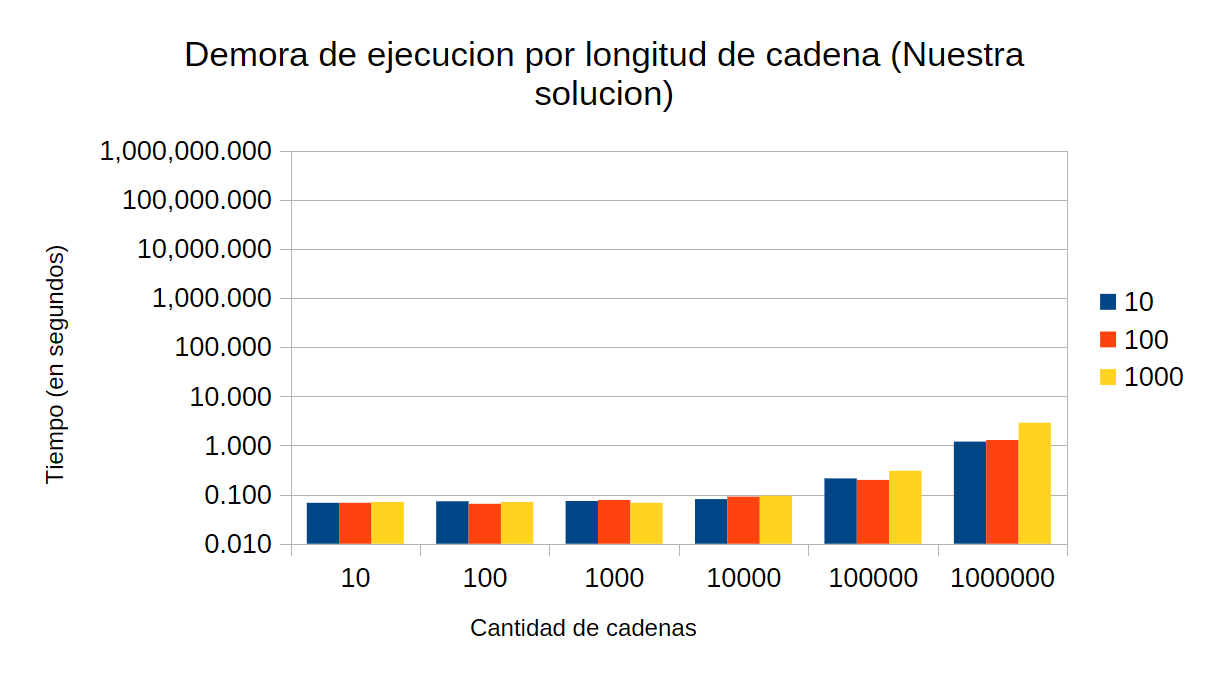
\includegraphics[width=0.5\linewidth]{nuestra_solucion.png}
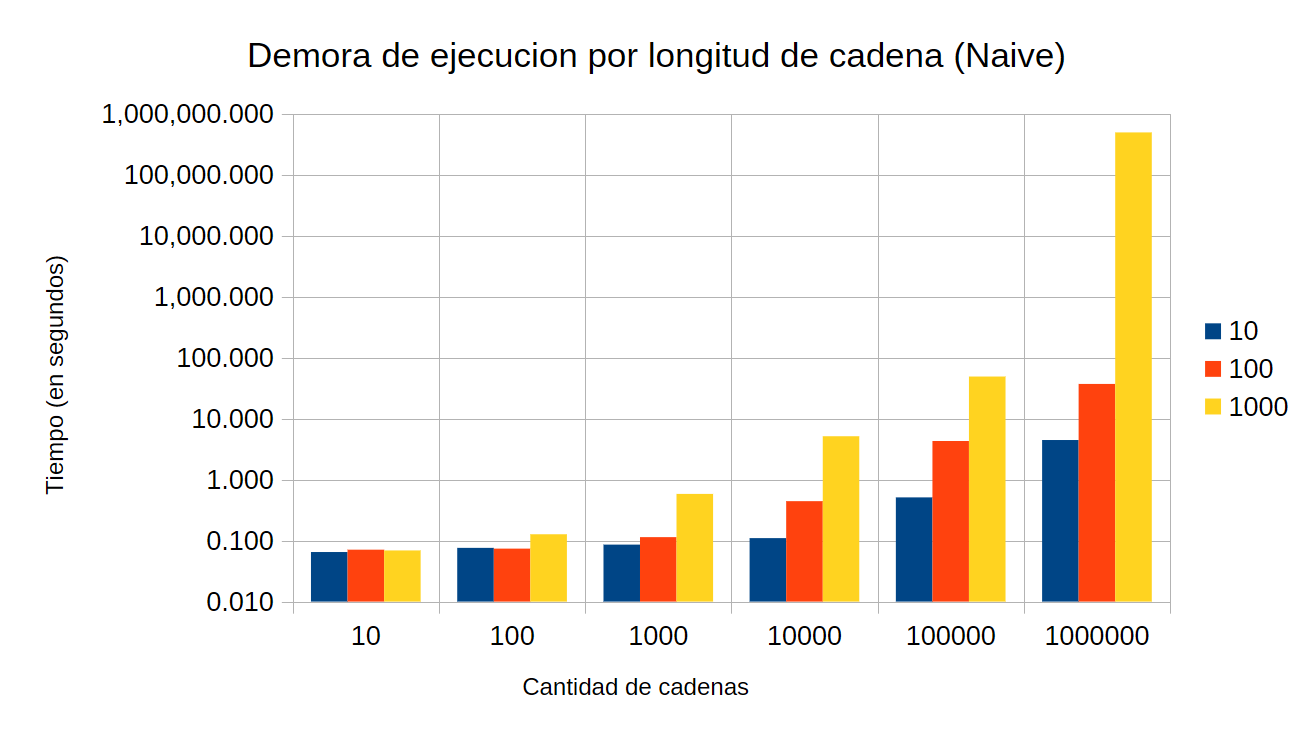
\includegraphics[width=0.5\linewidth]{solucion_naive.png}
\end{tabular}
\end{center}

En este gráfico los colores indican la longitud de las cadenas.

\section{Posibles mejoras}
Hay dos partes del código en los cuales tenemos una complejidad temporal que no es óptima, pero de todas formas se puede ver en los benchmarks que nuestra solución
es mejor que la naive. A continuación detallamos que partes son y cómo las mejoraríamos.

Al copiar los estados de un autómata vemos por cada uno si pertenece al conjunto de estados finales del autómata original, de la siguiente forma:
\begin{verbatim}
for state in states:
    afd.add_state(state, state in self.final_states)
\end{verbatim}
Esto es $O(|Q|^2)$, siendo $Q$ el conjunto de estados del autómata original. Esto lo podemos cambiar para que sea $O(n)$ normalizando los estados,
para que sean $q_0, q_1, \dots, q_{|Q|}$. Luego creamos un arreglo \verb|esFinal| de booleanos de longitud $|Q|$ inicializado en falso e iteramos cada $q_f \in F$
y marcamos su índice respectivo en \verb|esFinal|. Finalmente por cada $i$ tal que $0 \leq i \le |Q|$, agregamos el estado $q_i$ siendo final si $\verb|esFinal|[i]$
es verdadero.

En \verb|AFD| tenemos un método \verb|add_set_as_state| en el cual empezamos haciendo \verb|''.join(sorted(stateSet))|. Este método nos sirve para nombrar estados al 
determinizar y agregarlo al nuevo autómata finito, por ejemplo si se puede llegar a los estados $q_0, q_2$ y $q_3$, nombrará al nuevo estado \verb|"q0q2q3"|. Es necesario que
ordenemos el conjunto porque si no podemos representar un mismo estado en el afd con cadenas diferentes, en el ejemplo anterior también se podría nombrar al estado como \verb|"q2q0q3"|. El problema
es que hacer el sort del set de estados es $O(n \log{n})$, con $n$ siendo el tamaño del conjunto, si consideramos que comparar cadenas es constante, lo cual no es el caso. 
De todas formas se puede mejorar, primero asumiendo que los estados están normalizados, luego creando un arreglo con los índices que representan los estados que son enteros 
no negativos y haciendo counting sort sobre este en $O(n)$. Luego se puede convertir los numeros a strings y finalmente \verb|'q'.join(sortedArray)|. De esta forma pasamos
de $O(n \log{n})$ a $O(n)$.

